\documentclass[11pt]{article}
\usepackage{mathpazo}
\usepackage{url}
\usepackage{graphicx}
\usepackage{verbatim}

\newcommand{\spn}{\textsc{Spin}}
\newcommand{\prm}{\textsc{Promela}}
\newcommand{\js}{\textsc{jSpin}}
\newcommand{\spd}{\textsc{SpinSpider}}
\newcommand{\fil}{\textsc{FilterSpin}}
\newcommand{\dt}{\textsc{dot}}
\newcommand{\dtf}{\texttt{dot}}
\newcommand{\fsm}{\texttt{fsm}}
\newcommand{\p}[1]{\texttt{#1}}
\newcommand{\bu}[1]{\textsf{#1}}

\textwidth=15cm
\textheight=22cm
\topmargin=0pt
\headheight=0pt
\oddsidemargin=1cm
\headsep=0pt
\renewcommand{\baselinestretch}{1.1}
\setlength{\parskip}{0.20\baselineskip plus 1pt minus 1pt}
\parindent=0pt

\title{\js{} - Java GUI for \spn{}\\User's Guide\\\mbox{}\\\large{Version 5.0}}
\author{Mordechai (Moti) Ben-Ari\\
Department of Science Teaching\\
Weizmann Institute of Science\\
Rehovot 76100 Israel\\
\textsf{http://stwww.weizmann.ac.il/g-cs/benari/}}
%\date{}
\begin{document}
\maketitle
\thispagestyle{empty}

\vfill

\begin{center}
Copyright (c) 2003-10 by Mordechai (Moti) Ben-Ari.
\end{center}
Permission is granted to copy, distribute and/or modify this document
under the terms of the GNU Free Documentation License, Version 1.2
or any later version published by the Free Software Foundation;
with Invariant Section ``Introduction,'' no Front-Cover Texts, and no
Back-Cover Texts. A copy of the license is included in the file
\p{fdl.txt} included in this archive.
\newpage

\section{Introduction}

\subsection{\js{}}
\js{} is a graphical user interface for the \spn{} Model Checker that is
used for verifying concurrent and distributed programs. It is an
alternative to the \textsc{XSpin} GUI and was developed primarily for
pedagogical purposes. \js{} is written in Java, because the Java
platform is both portable and widely used in computer science education.
The user interface of \js{} is simple, consisting of a single window
with menus, a toolbar and three adjustable text areas. \spn{} option
strings are automatically supplied and the \spn{} output is filtered and
formatted. All aspects of \js{} are configurable: some at compile time,
some at initialization through a configuration file and some at runtime.
The filtering algorithm in \js{} can also be run as a standalone
program.

\subsection{\spd{}}
\js{} includes the \spd{} tool for creating a graphical representation for
the state diagram of a \prm{} program by postprocessor the \spn{} output. 
\spd{} is integrated into \js{}, but it can also be run as a standalone program.

\spd{} generates the complete state diagram of a \prm{} program; the 
diagrams are useful for demonstrating properties of concurrent programming.
Consider the \emph{third attempt} at solving the critical section problem (line
numbers added):
\begin{verbatim}
1.  bool wantp = false, wantq = false;
2.  
3.  active proctype p() {
4.      do :: wantp = true; 
5.            !wantq;
6.            wantp = false;
7.      od
8.  }
9.
10. active proctype q() {
11.     do :: wantq = true;
12.           !wantp;
13.           wantq = false;
14.     od
15. }
\end{verbatim}
The processes \p{p} and \p{q} are in their critical sections if they are at 
lines~6 and~13, respectively. The figure on the next page shows the state 
diagram for this program. Each node contains the source code lines (and line 
numbers) for the two processes and the values of the variables \p{wantp} and 
\p{wantq}. The arrows show the possible transitions between states. Since no 
state has the processes together at lines~6 and~13 mutual exclusion is 
achieved. It is easy to see there is a computation that leads to deadlock in 
the state with \p{p} at line~5 and \p{q} at line~15.
\begin{figure}[!htb]
\begin{center}
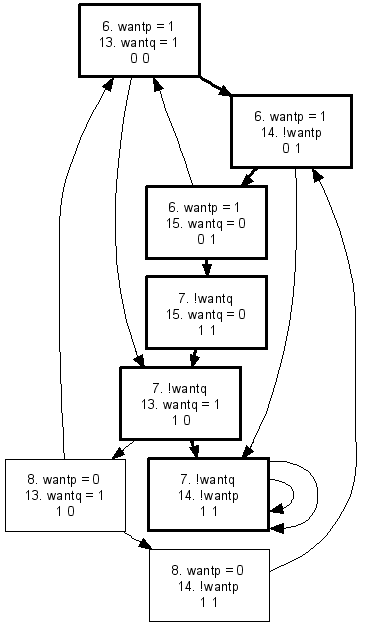
\includegraphics[width=6cm,keepaspectratio=true]{third.png}
\end{center}
\end{figure}

\spd{} processes output of the \p{pan} verifier in order to create the full 
state diagram of a program. The diagram is produced in \dtf{} format and 
(optionally) the \dt{} program can be run to produce a graphics file.
\spd{} can also produce state diagrams in \fsm{} format used by visualization 
tools developed at the Technische Universiteit Eindhoven (see the URLs below).

\subsection{References}
\begin{itemize}
\item M. Ben-Ari. \textit{Principles of the Spin Model Checker}. Springer, 2008.
\item M. Ben-Ari. \textit{Principles of Concurrent and Distributed Programming (Second
Edition)}. Addison-Wesley, 2006.
\item Gerard J. Holzmann. \textit{The Spin Model Checker: Primer
and Reference Manual}.\\Addison-Wesley, 2004.
\end{itemize}

\subsection{URLs}

\begin{tabular}{l@{\hspace{3em}}l}
\hline
\fsm{} & \url{http://www.win.tue.nl/~fvham/fsm/}\\
 & \url{http://www.mcrl2.org/}\\
\textsc{Graphviz (dot)} & \url{http://www.graphviz.org/}\\
\js{} & \url{http://stwww.weizmann.ac.il/g-cs/benari/jspin/}\\
\textsc{MinGW} & \url{http://mingw.org/}\\
\spn{} & \url{http://spinroot.com/}\\
\hline
\end{tabular}

\subsection{Acknowledgement}
I would like to thank Gerard J. Holzmann for his generous assistance throughout the
development of this project.

\section{Installation and execution}

\subsection{Requirements}
\begin{itemize}

\item \js{} requires that the Java SDK or JRE (at least version 1.5) be
installed.\footnote{The default font for \js{} is \p{Lucida Sans
Typewriter}. This font may no longer be available in the JRE you use. If
you have the fonts from a previous version you can copy them to the
\p{lib/fonts} directory as explained in
\url{http://java.sun.com/j2se/1.5.0/docs/guide/intl/font.html}.
Alternatively, you can change the configuration file to use a monospaced
font such as \p{Courier} that is installed by default.}

\end{itemize}

\subsection{Installation}
This section describes installation on a Windows system;
for custom installation and for other systems, see Appendix~\ref{a.install}.

\begin{itemize}
\item Download the \js{} installation file called \p{jspin-N.exe},
where \p{N} is the version number.
Execute the installation file.
\item Create a directory \verb=c:\mingw= and download the C 
compiler archive \p{mingw.exe} into that directory. Execute this self-extracting file.
\end{itemize}

\subsection{Configuring and running \js{}}
\begin{itemize}
\item The installation will create the following subdirectories: \p{docs} for the
documentation, \p{jspin} and \p{spinSpider} for the source files, 
\p{txts} for the text files
(help, about and copyright), and \p{jspin-examples} and \p{spider-examples}
for example programs.
\item To run \js{}, execute the command \p{javaw -jar jSpin.jar}.
An optional argument names the \prm{} file to be opened initially.
A batch file \p{run.bat} is supplied which contains this command.
\item Configuration data (Appendix~\ref{a.cfg}) is in the file
\p{config.cfg}.
\textbf{When upgrading \js{}, erase the configuration file before installing
a new version, so that new configuration options will be recognized.}
\item \js{} searches for the configuration file in the current
directory; if it is not found, \js{} searches for it in the directory
where the jar file is installed; if it is not found there, a new file
with default values is written.
\end{itemize}

\subsection{Running \spd{} without \js{}*}
If you want to run \spd{} without \js{}, create a configuration file
with entries for the \p{SPIN}, \p{C\_COMPILER}, \p{PAN} and \p{DOT}
commands. The prologues for the \dtf{} file can be changed in
\p{Config.java} in the package \p{spinSpider}.

The \p{SpinSpider} class has a main method that can be invoked from a command
line:
\begin{verbatim}
java -cp jSpin.jar spinSpider.SpinSpider arguments filename
\end{verbatim}
\p{filename} is the source file name. The arguments are:

\hspace*{1cm}
\begin{tabular}{ll}
\p{-pn} & The number of processes \p{n};\\
\p{-vname} & One parameter for each variable \p{name};\\
\p{-dot} & \dtf{} format;\\
\p{-Txxx} & \dtf{} format followed by conversion to \p{xxx} format,\\
& the default is \p{png};\\
\p{-fsm} & \fsm{} format;\\
\p{-t1} & Emphasize trail;\\
\p{-t2} & Display the trail only;\\
\p{-a} & Display automata for \prm{} source;\\
\p{-small} & Small size for states; if absent, large size is used;\\
\p{-bold} & Bold for emphasis; if absent, color is used.\\
\p{-debug} & Write debug file;\\
\end{tabular}\\
\noindent{}The \p{-p} and \p{-v} arguments must be given (unless \p{-a} is selected).

\subsection{Running \fil{} without \js{}*}
To run \fil{} from the command line, first create a file with the output
of a (random or guided) simulation:
\begin{verbatim}
   spin -p -l -g -r -s -X src.pml > src.raw
\end{verbatim}
Next, run \fil{}:
\begin{verbatim}
   java -cp jSpin.jar filterSpin.FilterSpin src.raw
\end{verbatim}
There are two optional arguments: \p{-v} to give a list of excluded
variables and \p{-s} to give a list of excluded statements, as described
in Section~\ref{s.filter}. The arguments may be file names or lists of
identifiers separated with a separator string (by default \p{"\#"}, but
it can be changed in \p{Config.java}\footnote{Do not use a backslash or
dollar sign.}). At least one separator must be given so that the
argument is not interpreted as a file name):
\begin{verbatim}
   java -cp jSpin.jar filterSpin.FilterSpin -v "temp#i" -s "i+1#" src.raw
\end{verbatim}
The filtered output is sent to standard output and can be piped or
redirected as needed. The configuration file must contain values for the
properties listed in Appendix~\ref{a.cfg} under \emph{filter settings}.

\section{\js{} Overview}
The user interface includes a menu, a toolbar and three text areas.
Menu and toolbar commands have keyboard mnemonics or accelerators.
These can be easily configured by modifying the file \p{Config.java} and
rebuilding.

The left text area is used to display \prm{} source files. The bottom
text area is used to display messages from both \spn{} and \js{}. The
right text area is used to display the output from \spn{}: statements
executed, values of variables and results of verifications. The text
areas can be resized by dragging the dividers and an area can be hidden
by clicking on the triangles in the dividers; the initial sizes can be
set in the configuration file. The toolbar button \bu{Maximize} (with
its mnemonic \bu{Alt-M}) toggles between a normal split pane and a
maximized right text area that displays the \spn{} output.

\begin{figure}[tb]
\begin{center}
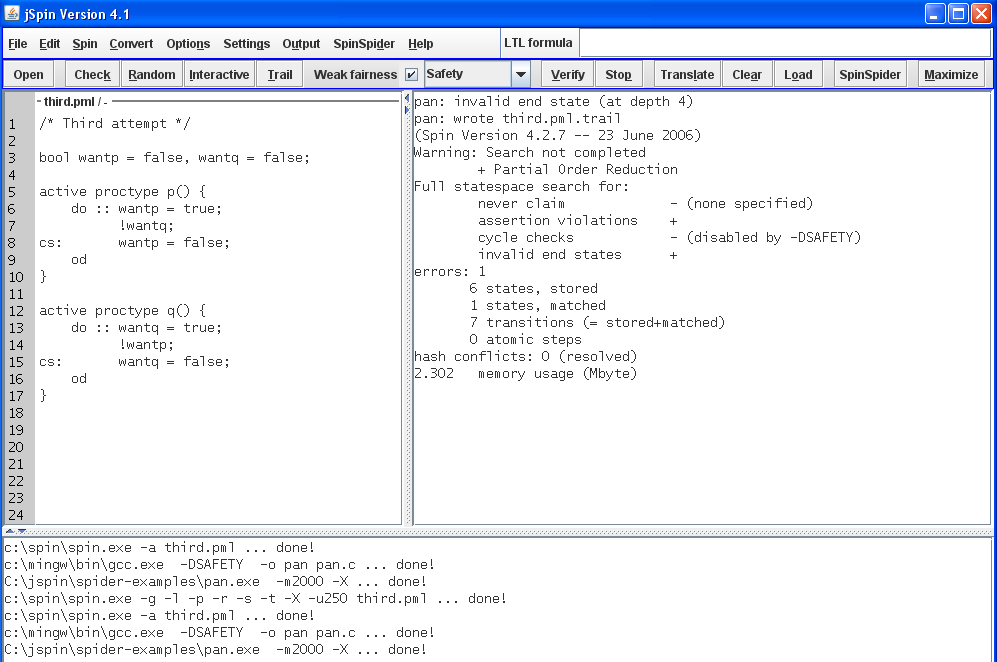
\includegraphics[width=140mm]{jspin.png}
\end{center}
\end{figure}

\begin{description}
\item[\bu{File}] This menu includes selections for \bu{New}, \bu{Open}, 
\bu{Save}, \bu{Save As}, and \bu{Exit}. \bu{Switch file} closes the 
current file and opens the last file that was edited, if any. This is 
useful for working with both a source file and an included file.

\item[\bu{Edit}] This menu includes selections for \bu{Undo}, \bu{Redo}, 
\bu{Copy}, \bu{Cut}, \bu{Paste}, \bu{Find} and \bu{Find again}.

\item[\bu{Options}] This menu enables you to edit the option strings for 
each of the phases of execution of \spn{} and the C compiler. Normally, you
will not need to change the options except for those that are more
conveniently changed in \bu{Options/Common} or \bu{Settings}
(Section~\ref{s.run}). \bu{Default} restores the default 
values and \bu{Save} saves the current set of option strings in the 
configuration file. In addition, the following configuration items are
automatically saved:
\begin{itemize}
\item \p{SOURCE\_DIRECTORY}: the last directory from which a source file was opened.
\item The current values of the splitpane dividers \p{TB\_DIVIDER} and
\p{LR\_DIVIDER}.
\item The current value of the width \p{SELECT\_BUTTON} for interactive
simulation.
\end{itemize}
The file can be saved
to the \bu{current} or \bu{install} directory. \textbf{Changes in the
\spn{} options can cause the assumptions on the input to \p{filter} to
become falsified. Be careful!}

\item[\bu{Settings}] This menu sets parameters for the simulation and 
verification (Section~\ref{s.run}).

\item[\bu{Output}] This menu controls the display of the simulation output
in the right text area. \bu{Output/Maximize} toggles the text area to be
maximized, hiding the editing area. \bu{Output/Save output} saves the
contents of the text area in a file with extension \p{.out}.
To debug the filtering algorithm,
select \bu{Output/Raw output} to write a file with extension
\p{.raw} that contains the raw \spn{} output;
\bu{Output/Display raw} will display this file.
The other items in this menu are discussed in Section~\ref{s.run}.

\item[\bu{SpinSpider}] This menu enables interactive execution of the \spd{} 
tool for creating graphical representations for the state diagram of a 
\prm{} program. See the separate documentation for this tool.

\item[\bu{Help}] \bu{Help} displays a short help file and \bu{About} 
displays copyright information about the software.
\end{description}

\section{Running \spn{}}\label{s.run}
In the \bu{Spin} menu (and on the toolbar) are five selections for
running \spn{}. They all use the \prm{} source file that has been opened,
and save the file before execution.
During simulation and verification,
you can select \bu{Stop} to terminate the \spn{} process that has been forked.
\begin{description}
\item[\bu{Check}] Runs a \emph{syntax check}.
\item[\bu{Random}] Runs a \emph{random simulation}.
\item[\bu{Interactive}] Runs an \emph{interactive simulation}.
\item[\bu{Guilded}] Runs a \emph{guided simulation} using the trail
file created by the execution of the analyzer.
\item[\bu{Verify}] Runs an \emph{verification}.
\end{description}
\textbf{If you terminate \js{} while \spn{} is running (for example by entering \bu{ctrl-C} from the
command line), make sure to terminate the \spn{} process as well.}\\
In Windows this is done by pressing \bu{ctrl-alt-del}, followed by
selecting \bu{Task List} and \bu{Processes}. Select \bu{spin.exe} and
\bu{End Process}.

\subsection{Simulation}\label{s.sim}
\bu{Check} should be run before any simulation run to ensure better display
of errors.

\bu{Settings/Max steps} changes the \p{-u} option to limit the number of
simulation steps, and \bu{Settings/Max depth} changes the \p{-m} option
to limit the \p{pan} search depth.

A nonzero value for \bu{Settings/Seed} will be used as the seed for generating
random numbers, enabling a random simulation to be repeated.

\subsubsection{Interactive simulation}
During an interactive simulation, a dialog frame will pop up with a list
of statements that can be executed. The list can be displayed either as
a row of buttons, or---if there is not enough room---as a pulldown menu.
The choice of the format is dynamically determined according to the
value of the configuration option \p{SELECT\_MENU}. By setting this
value to an extreme, you can force the list to a certain format. There
are also configuration options for setting the width and height of the
buttons or menu items.

The dialog can be navigated using the mouse; closing the dialog frame
will terminate interactive simulation. For keyboard navigation:
\begin{description}
\item[Buttons] \bu{Tab} and \bu{Shift-Tab} move through the buttons
and \bu{Space} selects the highlighted button. Press \bu{Esc} to terminate.
\item[Menu] Press down arrow to display the list and to highlight the
item you want; press \bu{Return} to select it. Press \bu{Esc} to terminate.
\end{description}

\subsubsection{Filtered output}\label{s.filter}
The contents of the \spn{} output can be changed by selecting 
\bu{Options/Common}. This pops up a dialog with check boxes to select the 
\spn{} output options: statements (\p{-p}), local variables (\p{-l}), 
global variables (\p{-g}), messages sent (\p{-s}) and messages received 
(\p{-r}). 

Select \bu{Output/Exclude variables} to create a list of strings defining 
variables to be \emph{excluded} from the display. Any variable containing 
a string from the list is not displayed; for example, \p{:init:} will 
exclude all variables of the \p{init} process. If the variable name is 
prefixed by \p{+}, it will be included anyway. For exmple, if you have an 
array variable \p{test}, then the entries \p{test} and \p{+[1]} will 
exclude display of the elements of \p{test} except for \p{test[1]}. The 
list is saved on a file with extension \p{.exc}.

Similarly, a file of excluded statements can be created. The file 
extension is \p{.exs} and it may be edited by selecting \bu{Output/Exclude 
statements}. \bu{Exclude statements} should \emph{not} be used with 
interactive simulation.

The output strings from \p{printf} statements is displayed normally. Optionally,
you can request that only strings beginning with \p{MSC:} be displayed (\p{MSC=true}).

\subsection{Verification}
Selecting \bu{Spin/Verify} or the \bu{Verify} button on the tool bar
performs the three steps required to verify a \prm{} program in \spn{}:
\begin{itemize}
\item Run \spn{} to create an analyzer in files \p{pan.*}.
\item Run the C compiler to compile the analyzer \p{pan.c}.
\item Run the analyzer \p{pan.exe}.
\end{itemize}
There are three modes of verification in \spn{},
one of which must be selected from the combo box on the toolbar
or the radio buttons in the menu \bu{Settings}:
\begin{description}
\item[Safety] Checks basic safety properties such as assertions.
\item[Acceptance] Checks for acceptance cycles.
\item[Non-Progress] Checks that every cycle contains a
\p{progress} label.
\end{description}
See the \spn{} reference manual for descriptions of these modes.
Checking \bu{Weak fairness} in the menu \bu{Settings}
or on the toolbar performs the verification only for executions that are
weakly fair.

\subsection{LTL formulas}\label{s.ltl}

A correctness claim specified by a \emph{Linear Temporal Logic (LTL)}
formula must be converted to an automaton written as a \prm{} \p{never}
claim. LTL formulas can be contained within the \prm{} source code or
they can be placed in external files.

\subsection{Internal formulas}

An LTL formula can be included in a \prm{} program:
\begin{verbatim}
ltl { []<>csp && []<>csq }
\end{verbatim}
The formula is translated internally by \spn{} into a \p{never} claim.

A number of \emph{named} formulas can be included within a \prm{} program:
\begin{verbatim}
ltl p0 { [](gate <= 1) }
ltl p1 { []((count == 0) -> (gate == 0)) }
ltl p2 { [](((gate == 0) && notInTest) -> (count == 0)) }
\end{verbatim}
To select which claim will be used in a verification, enter the
\emph{name} in the \bu{LTL formula} text field and select \bu{LTL name}.

The above examples show that internal LTL formulas can have expressions
and not just names as atomic propositions.

\textbf{\spn{} automatically negates LTL formulas contained within a
\prm{} program.}

\subsubsection{External formulas}

Enter a formula (such as \p{[]p} or \p{<>p}) in the text field labelled
\bu{LTL formula} on the menu bar and select \bu{Translate} from the
toolbar or the \bu{Convert} menu; the formula translated into a
\p{never} claim which will be added to the next \spn{} verification. The
\p{never} claim is stored in a file with extension \p{.ltl}. The formula
is not automatically translated, so whatever \p{never} claim exists, if
any, will continue to be used until \bu{Translate} is invoked again.

\textbf{Before the formula is translated it is negated by \js}. This is
done so that the LTL formula as displayed represents the correctness
property being checked and not the negated formula which if satisfied
represents a counterexample. Should you wish to enter negations yourself
as in \spn{}, you can change the configuration file option
\p{NEGATE\_LTL} to false; this can also be done by toggling
\bu{Settings/Negate LTL}.

LTL formulas are saved in \emph{property files} with extension \p{.prp}.
By default, when you open a \prm{} file,
\js{} opens and loads a \p{.prp} file of the same name.
You can also load a different file by selecting \bu{Load} from
the toolbar or the \bu{Convert} menu;
the file name will be displayed on the toolbar.
If the file does not exist,
the text field is cleared and the new name is used when you \bu{Translate} the formula
you enter.

The property file is saved whenever the source file is
and also before translation.

\bu{Convert/Clear} not only to clears the text field, but ensures that
no LTL formula will be used in the next verification. After selecting
\bu{Convert/Clear} an empty file will not be saved. Note: In earlier
versions of \js{}, a button \bu{Clear} was available on the toolbar;
this has now been removed and the menu selection must be used.

\section{\spd{}}
Open a \prm{} program. If you wish to emphasize or draw the computation
described by a \p{trail} file, execute \spn{} in verification mode with
appropriate assertions or LTL formulas to create the trail file for a counterexample.

Select \bu{SpinSpider/SpinSpider} (\bu{ctrl-D}) from the menu or \bu{SpinSpider}
from the toolbar and the following frame will appear:
\begin{center}
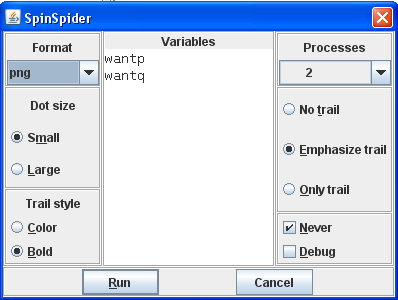
\includegraphics[width=9cm,keepaspectratio=true]{spd.png}
\end{center}
\begin{description}
\item[\bu{Format}] The output format, normally \bu{dot} or one of the formats
such as \bu{png} that can be obtained by running \dt{}. The \bu{fsm} format is
experimental and the processing of the trail file is not done for this format.
\textbf{If \p{png} is selected as the format, the state diagram will be displayed in a
separate frame when \spd{} has terminated.}
\item[\bu{Processes}] The number of processes in the program (for generation of
the \p{never} claim).
\item[\bu{Variables}] A list of the variables in the program (for generation of
the \p{never} claim).
\item[\bu{No trail}, \bu{Emphasize trail}, \bu{Only trail}] If the first option
is selected, the entire state diagram is created. The second option colors nodes
and edges in the state diagram that are part of the trail. The third option
creates a diagram containing only those states and nodes that are part of the
trail.
\item[\bu{Automata}] This displays the source of the \prm{} program as a set
of automata, one for each \p{proctype}; for the \emph{third attempt}, this is:
\begin{center}
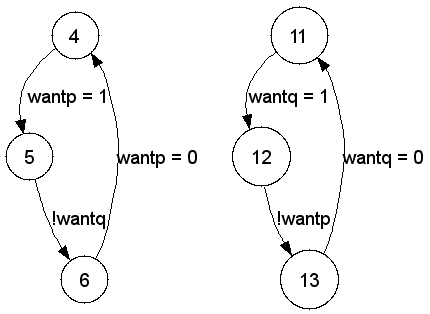
\includegraphics[width=7cm,keepaspectratio=true]{third-automata.png}
\end{center}
The states are labeled with the source code line numbers and the edges with
the statements associated with each transition. \p{atomic} transitions
are emphasized.
\item[\bu{Dot size}] Chooses between two prologues for the \dtf{} file. The small
option works better for display within \js{}.
\item[\bu{Trail style}] Chooses between two ways of emphasizing the trail in a
computation: in color or bold. The latter is useful for including the diagram in
a document or for users with difficulty seeing colors.
\item[\bu{Debug}] Writes a file (extension \p{.dbg}) with the internal data
structures as collected from the execution of \spn{}: states, transitions,
statements and the trail. 
(The file is automatically generated if \bu{Automata} is selected.) 
This file can be displayed by selecting
\bu{SpinSpider/Display debug} from the \js{} menu.
\item[\bu{Run}] Saves the current parameters in a file with the same name as the
source file and with extension \p{.spd}. Then \spd{} is run.
\item[\bu{Cancel}] Returns without saving the parameters or running \spd{}.
\end{description}

\subsection{\prm{} programs for \spd{}}
The directory \bu{spider-examples} contains concurrent programs that demonstrate
the use of \spd{}.

To reduce the size of the diagrams, use \emph{remote references} rather than
ghost variables in the specification of correctness properties. For example, to
prover that mutual exclusion holds in the third attempt (\p{third.pml}), declare
labels \p{cs:} at the two critical sections and then define the symbol:
\begin{verbatim}
#define notmutex (p@cs && q@cs)
\end{verbatim}
Mutual exclusion can shown by doing a verification in \bu{Safety} mode
with the LTL formula:
\begin{verbatim}
!<>notmutex
\end{verbatim}
Recall that \spn{} finds the \emph{first} counterexample in a depth-first
search, not the shortest one. The trail for the program for the fourth
attempt (\p{fourth.pml}) was created by running \p{pan} with the \p{-i}
parameter to do an iterative search for a short counterexample.

The line numbers will be accurate if the first alternative of a \p{do}- or 
\p{if}-statement is written on the same line as the keyword. Note that all 
alternatives are considered to belong to the line containing the keyword.

%\newpage

\section{Troubleshooting}
\begin{description}
\item[\spn{} won't execute] Check the configuration items
for \spn{} and the C compiler.
It is recommended that they be in your path.
\item[Exceptions in Filter] Your own output might be
interfering with the filtering algorithm.
If configuration option \p{MSC} is selected, use \p{printf} only with strings
prefixed by \p{MSC:} and terminated by a newline.
\item[Verification doesn't seem to work]
Make sure that you have selected the appropriate mode
from the \bu{Settings} menu:
\bu{Safety}, \bu{Acceptance}, \bu{Non-progress}.
If you are using an LTL formula,
\bu{Translate} it before verifying.
\item[Your computer works slowly] Forked processes for \spn{} are still executing.
Terminate them from the operating system.
\item[Settings, options and the directory aren't remembered]
You must select \bu{Options/Save} before exiting \spn{}.
\item[Preprocessing failed] Simple preprocessing like the use of \verb=#define= 
is done internally by \spn{}. For more complicated processing, \spn{} calls the 
C compiler's preprocessor. This error message can result if there is a problem
with the installation; check also that the C compiler is in the path.
To debug preprocessing, execute \spn{} with the argument \p{-I};
this will perform preprocessing only on the \prm{} file and display the result. 
\end{description}

\newpage

\section{Software structure*}
The software is divided into three Java packages.

\subsection{Package \p{jspin}}
\p{jSpin} is the main class and contains declarations
of the GUI components and instances
of the classes \p{Editor} and \p{RunSpin}.
Method \p{init} and the methods it calls initialize the GUI.
Method \p{action\-Per\-formed} is the event handler for all the menu items
and buttons; it calls the appropriate methods for handling each event.
The \bu{About} and \bu{Help} options are implemented by reading files
\p{copyright.txt} and \p{help.txt}, respectively, and displaying
them in a \p{JFrame} with a scrollable \p{JTextArea}.

\p{JSpinFileFilter} is used with a \p{JFileChooser}
when opening and saving files: \prm{} source files,
LTL property files and \spn{} display output files.

\p{Options} is the dialog frame with check boxes for
changing the \spn{} display options.

\p{Exclude} is the dialog frame for editing the list
of variable strings to be excluded from the display.

\p{Config} contains declarations of compile time configuration items.
Method \p{init} calls \p{set\-Default\-Properties} to initialize the instance
of \p{Properties} with the default values of the dynamic configuration
items; it then attempts to load the configuration file, and if unsuccessful,
the default properties are written to a new file.

\p{Editor} implements an editor using operations on a
\p{JTextArea}. It implements the interface \p{Document\-Listener} to flag
when the source has been modified. The class is also responsible
for the LTL formula \p{JTextField}. \p{jSpin} calls method \p{writeFile}
to write \p{ltl} and \p{out} files, and method \p{readFile} to read
the text files to be displayed.

\p{LineNumbers} extends a \p{JComponent} to create line numbers
for the \p{RowHeaderView} of the editor \p{JScrollPane}
(thanks to Niko Myller for this code).

\p{UndoRedo} was extracted from an example on the Java web site.

The event handler in \p{jSpin} calls \p{run} in class \p{RunSpin}
to execute \spn{}, the C compiler and the analyzer \p{pan}.
\p{run} creates a thread of class \p{RunThread},
and uses \p{ProcessBuilder} to set up the
command, directory, merge the output and error streams,
and set up streams for I/O.
The call \p{runAndWait} is used for short calls like \bu{Check}
and the creation and compilation of a model;
this call does not return until the completion of the subprocess.
The call \p{run} will return immediately after it has created the thread.
In this case, the event handler in \p{jSpin} calls \p{isSpinRunning}
to create a thread to poll for termination of \spn{};
by creating a separate thread, the event handler is freed to accept
a selection of \bu{Stop}.

When \p{Select a statement} is received during an interactive simulation,
method \p{select} is called.
This method displays the choices in the bottom text area and pops up a
dialog to enable the user to make a selection.
A \p{JFrame} is created in a new thread of the inner class \p{SelectDialog} to wait
for the selection.
\p{select} polls \p{selectedValue} which is set with the selected button
value or zero if the frame is closed or \bu{Esc} pressed.
In that case, \p{q} is sent to \spn{} to terminate the simulation.

\js{} contains source code for interactively invoking \spd{}.
The class \p{SpiderOptions} pops up frame where parameters can be entered and
\spd{} invoked. Each \prm{} file can have its own set of parameters; these are stored
in property files with extension \p{.spd} and managed by \p{SpiderFile}. 
If the diagram is created in \bu{PNG} format, it is displayed interactively:
\p{DisplayImage} creates a frame and 
the image is loaded into an instance of \p{ImagePanel}.

\subsection{Package \p{filterSpin}}

The output filtering is encapsulated in class \p{Filter}.
For each line received from the output stream, \p{run}
(of \p{RunThread}) calls \p{filter}
which modifies the string; the modified string is displayed in the
appropriate text area.
A \p{TreeMap} is maintained for mapping variable names into value strings.
Each new variable is checked against the list of excluded strings before
it is entered in the map.
For standalone filtering, the package 
contains a \p{Config} class and a class \p{FilterSpin} with a main method.

\subsection{Package \p{spinSpider}}

Most of the processing of the \spd{} program is done 
in the class \p{SpinSpider}. 
Static data like strings and the prologue for the \dtf{} file are
contained in the class \p{Config}. 

Four classes are used for
objects containing information extracted from the files:
\begin{itemize}
\item \p{State} contains the program counter values and the variables names
and values that are extracted from the output of the \p{never} claim in the
\p{.chk} file.
\item \p{Transition} contains the transitions and is obtained by following
the \p{New}, \p{Old}, \p{Up} and \p{Down} debugging trace in the \p{.chk} file.
A stack is used to simulate the depth-first search of \spn{}.
\item \p{Statement} contains the states, line numbers and source statements
from the \p{.d} file.
\item \p{Trail} contains the \p{id} of an entry in the trail file.
\end{itemize}
The processing sequence is invoked from the method \p{runSpider}. 
\p{runProcess} is called several times to fork processes as described in
Section~\ref{s.how}. The \p{.d} file is analyzed in \p{createStatements},
and the \p{.chk} file is analyzed in \p{readCheckFile} of class \p{Read}.
If requested, these data structures are written to a file in method 
\p{writeDebug} of class \p{Write}.

The class \p{SetTrail} traverses the state diagram according to the trail and
marks states and transitions that are part of the trail.

The data structures are used to write the files in class \p{Write}.
See the description of the \fsm{} format to understand \p{writeFSMGraph}.
In \p{writeDOTGraph}, the \p{states} array is traversed sequentially 
writing out numbered nodes including labels for each node. The 
elements of this array store the program counters of each process in the 
state; these are used to search the \p{statements} array for \emph{all} 
statements that start from the program counter. The line numbers and 
source code of the statements are appended to the label. The variable 
values are also obtained from the \p{states} array. The transitions are
taken directly from the \p{transitions} array. Finally, \dt{} is called, if
requested.

The class \p{DrawAutomata} uses the information in the \p{.d} file
to write a \dtf{} file and then calls \dt{}.

\subsection{How \spd{} works}\label{s.how}

\spd{} works with numerous files:
\begin{itemize}
\item The source file with extension \p{.pml}.
\item A \p{never} claim file with extension \p{.nvr} as described below;
this is normally generated automatically.
\item The file with extension \p{.chk} obtained by running a verification of 
the program with the \p{-DCHECK} option and with the \p{never} claim that 
prints out the program counters and variable values.
\item The statement file with extension \p{.d} obtained by running a verification
with the \p{-d} option.
\item A file with extension \p{.spd} that is used by \js{} to save \spd{} parameters.
\item A debug file with extension \p{.dbg}.
\end{itemize}

\spd{} runs the following commands in subprocesses (\p{prog.pml} is the source file):

\hspace*{1cm}\p{spin -a prog.pml}\\
\hspace*{1cm}\p{gcc -DCHECK -DSAFETY -DPRINTF -o pan pan.c}\\
\hspace*{1cm}\p{pan > prog.chk}\\
\hspace*{1cm}\p{pan -d > prog.d}

Then it runs its own algorithm to create a \dtf{} file. Finally, \dt{} is 
optionally run to create a display file in some format like \p{png}.

A \prm{} program must be modified by giving a special \p{never} claim; this is
generated automatically and included using the \p{-N} argument to \spn{}. 

The \p{never} claim contains a single \p{printf} statement in a loop, which is 
executed with every step of the verifier. The statement prints the 
following tokens separated by spaces:
\begin{itemize}
\item The string \p{*spd*};
\item The number of processes, followed by the values of \p{pc\_value}
for each process;
\item The number of variables, followed by their names and values.
\end{itemize}
For the algorithm shown in the introduction the \p{never} claim is:
\begin{verbatim}
never {
  do :: printf("*spd* 2 %d %d 2 wantp %d wantq %d \n",
        pc_value(0), pc_value(1), wantp, wantq)
  od
}
\end{verbatim}

\newpage

\appendix

\section{Installation}\label{a.install}

\subsection{\spn{} version}

Version 6.0.0 of \spn{} changed its output format; starting with version
5.0, \js{} expects this format. You can still run \js{} with earlier
versions of \spn{} (for example, 4.30): set the configuration option
\p{VERSION} to a number less than 6 before you run \js{} and ensure that
the option \p{SPIN} names the earlier version of the \spn{} executable
(or copy the file over the later version).

\subsection{Custom installation of \js{}}
\begin{itemize}
\item Download the \js{} distribution file called \p{jspin-N.zip},
where \p{N} is the version number.
Extract the files into a clean directory.
%\textbf{Do not} install to a directory with spaces like \verb=c:\Program Files=.

\item Install \spn{} and \textsc{dot} (\textsc{dot} is only needed for
\textsc{SpinSpider}).

\item Install an ANSI C compiler.

\item Modify the configuration file \p{config.cfg} to reflect the
locations of the programs.
\end{itemize}

\subsection{Building \js{}}

To rebuild \js{}, execute \p{build.bat}, which will compile all the source
files and create the file \p{jSpin.jar} with the manifest file.

\subsection{Installing a C compiler}\label{a.c}
The \p{gcc} compiler is normally used with \spn{}. On Windows, there are
two distributions: Cygwin (\url{http://cygwin.com}) is a comprehensive
Linux-like environment, and a smaller distribution called MinGW
(\url{http://mingw.org/}). To install MinGW, download the following archives and
open them in directory \verb=c:\mingw= \emph{in the following order}:
\begin{quote}
\p{binutils-V.tar.gz}\\
\p{gcc-core-V.tar.gz}\\
\p{mingw-runtime-V.tar.gz}\\
\p{w32api-V.tar.gz}
\end{quote}
where V is the version and build number.
It is OK if some files are overwritten when opening the archive.

Set the path in
\begin{quote}
\p{Start/Control Panel/System/Advanced/Environment Variables/PATH}
\end{quote}
to include \verb=c:\mingw\bin=.

\subsection{Installing \js{} on \textsc{Mac OS X}}\label{a.mac}

Thanks to Christiaan Ottow for providing this material.

Currently, there is no precompiled version of \spn{}, so you will have to
compile it from the source code. Instructions for doing this are given
in Section~2c of the webpage:
\begin{quote}
\url{http://spinroot.com/spin/Man/README.html}
\end{quote}
An alternative approach is change the location of the preprocessor specified in 
lines 75--88 of \p{main.c} from \p{/lib/cpp} to \p{/usr/bin/cpp}.

\js{} is compiled with \p{-target 1.5} to conform with the \textsc{Java}
version currently available on the \textsc{Mac}.

To install \js{}:
\begin{itemize}
\item Unzip the file \p{jspin-V-V.zip}.
\item Download \textsc{Graphviz} from
\begin{quote}
\url{http://www.pixelglow.com/graphviz/download}
\end{quote}
Open the \p{dmg} file you downloaded and copy the \textsc{Graphviz}
application to the Applications folder.
\item Open the configuration file \p{config.cfg} in a text editor and change the
values of the following properties: 
\begin{itemize}
\item \p{SPIN} to the directory with the compiled \spn{};
\item \p{SOURCE\_DIRECTORY} to the subdirectory \p{jspin-examples} of the directory
where you unpacked \js{};
\item \p{C\_COMPILER} to directory containing \p{gcc},
usually \p{/usr/bin/gcc}. You can verify this by issuing the command \p{which gcc};
\item \p{PAN} to \p{pan};
\item \p{DOT} to \p{/Applications/Graphviz.app/Contents/MacOS/dot}.
\end{itemize}
\end{itemize}

\js{} can now be run by using the \p{Terminal} to execute the following command
in the \p{jspin} directory:
\begin{quote}
\p{java jspin.jSpin} 
\end{quote}

\subsection{Installing \js{} on \textsc{Linux}}\label{a.linux}

Thanks to Vsevolod Krishchenko for providing this material.

\begin{itemize}

\item Install gcc, C preprocessor, dot, java. For Debian/Ubuntu:
\begin{verbatim}
  sudo apt-get install gcc cpp graphviz sun-java6-jre
\end{verbatim}
\item Install spin as described above.
\item Make the following changes in \p{config.cfg}:
\begin{verbatim}
  C_COMPILER=gcc
  DOT=dot
\end{verbatim}
You many need to set \p{SINGLE\_QUOTE} to \p{true}.
\item Create a shell file with:
\begin{verbatim}
  #!/bin/sh
  java -jar jSpin.jar
\end{verbatim}
\end{itemize}

\section{Configuration file}\label{a.cfg}

These tables give the properties in the configuration file and their
default values.

\begin{center}

\begin{tabular}{|p{.3\textwidth}|p{.4\textwidth}|}
\hline
\multicolumn{2}{|c|}{Version of \spn{}}\\ \hline
\textsc{\ttfamily VERSION} &\verb+6+\\\hline
\end{tabular}

\bigskip

\begin{tabular}{|p{.3\textwidth}|p{.4\textwidth}|}
\hline
\multicolumn{2}{|c|}{Directories for source and compilers}\\ \hline
\textsc{\ttfamily SOURCE\_DIRECTORY} & \verb+"jspin-examples"+ \\
\textsc{\ttfamily C\_COMPILER} &\verb+"c:\\mingw\\bin\\gcc.exe"+ \\
\textsc{\ttfamily SPIN} &\verb+"bin\\spin.exe"+ \\
\textsc{\ttfamily DOT} &\verb+"bin\\dot.exe"+ \\
\textsc{\ttfamily PAN} &\verb+"pan"+ \\ \hline
\end{tabular}

\bigskip

\begin{tabular}{|p{.3\textwidth}|p{.4\textwidth}|}
\hline
\multicolumn{2}{|c|}{Options for executing \spn{}}\\ \hline
\textsc{\ttfamily COMMON\_OPTIONS} &\verb+"-g -l -p -r -s"+\\
\textsc{\ttfamily CHECK\_OPTIONS} &\verb+"-a -v"+\\
\textsc{\ttfamily RANDOM\_OPTIONS} &\verb+"-X"+\\
\textsc{\ttfamily INTERACTIVE\_OPTIONS} &\verb+"-i -X"+\\
\textsc{\ttfamily VERIFY\_OPTIONS} &\verb+"-a"+\\
\textsc{\ttfamily C\_COMPILER\_OPTIONS} &\verb+"-o pan pan.c"+\\
\textsc{\ttfamily PAN\_OPTIONS} &\verb+"-X"+\\
\textsc{\ttfamily TRAIL\_OPTIONS} &\verb+"-t -X"+\\
\textsc{\ttfamily TRANSLATE\_OPTIONS} &\verb+"-f"+\\
\textsc{\ttfamily MAX\_STEPS} {\ttfamily (-u)} &     \verb+250+\\
\textsc{\ttfamily MAX\_DEPTH} {\ttfamily (-m)} &     \verb+2000+\\
\textsc{\ttfamily SEED} {\ttfamily (-n)} &     \verb+0+\\
\textsc{\ttfamily FAIRNESS} &      \verb+true+\\
\textsc{\ttfamily RAW} & \verb+false+\\
\textsc{\ttfamily SINGLE\_QUOTE} &      \verb+false+\\
\textsc{\ttfamily NEGATE\_LTL} &      \verb+true+\\
\textsc{\ttfamily VERIFY\_MODE} &   \verb+"Safety"+\\\hline
\end{tabular}

\bigskip

\begin{tabular}{|p{.3\textwidth}|p{.4\textwidth}|}
\hline
\multicolumn{2}{|c|}{Filter settings}\\ \hline
\textsc{\ttfamily PROCESS\_TITLE} & \verb+Process +\\
\textsc{\ttfamily PROCESS\_WIDTH} & \verb+7+\\
\textsc{\ttfamily STATEMENT\_TITLE} & \verb+Statement +\\
\textsc{\ttfamily STATEMENT\_WIDTH} & \verb+18+\\
\textsc{\ttfamily VARIABLE\_WIDTH} &\verb+10+\\
\textsc{\ttfamily LINES\_PER\_TITLE} &\verb+20+\\
\textsc{\ttfamily MSC} &\verb+false+\\
\hline
\end{tabular}

\bigskip

\begin{tabular}{|p{.3\textwidth}|p{.4\textwidth}|}
\hline
\multicolumn{2}{|c|}{Text settings}\\ \hline
\textsc{\ttfamily WRAP} &\verb+true+\\
\textsc{\ttfamily TAB\_SIZE} &\verb+4+\\
\textsc{\ttfamily FONT\_FAMILY} & \verb+"Lucida Sans Typewriter"+\\ 
\textsc{\ttfamily FONT\_STYLE} & \verb+java.awt.Font.PLAIN+\\
\textsc{\ttfamily FONT\_SIZE} & \verb+14+\\\hline
\end{tabular}

\bigskip

\begin{tabular}{|p{.3\textwidth}|p{.4\textwidth}|}
\hline
\multicolumn{2}{|c|}{Frame size}\\ \hline
\textsc{\ttfamily WIDTH} &\verb+1000+\\
\textsc{\ttfamily HEIGHT} &\verb+700+\\\hline
\end{tabular}

\bigskip

\begin{tabular}{|p{.3\textwidth}|p{.4\textwidth}|}
\hline
\multicolumn{2}{|c|}{Interactive dialog settings}\\ \hline
\textsc{\ttfamily SELECT\_BUTTON} &\verb+120+\\
\textsc{\ttfamily SELECT\_HEIGHT} &\verb+70+\\
\textsc{\ttfamily SELECT\_MENU} &\verb+5+\\\hline
\end{tabular}

\bigskip

\begin{tabular}{|p{.3\textwidth}|p{.4\textwidth}|}
\hline
\multicolumn{2}{|c|}{Location of dividers}\\ \hline
\textsc{\ttfamily LR\_DIVIDER} &\verb+400+\\
\textsc{\ttfamily TB\_DIVIDER} &\verb+500+\\
\textsc{\ttfamily MIN\_DIVIDER} &\verb+50+\\\hline
\end{tabular}

\bigskip

\begin{tabular}{|p{.3\textwidth}|p{.4\textwidth}|}
\hline
\multicolumn{2}{|c|}{Delay while waiting for user input}\\ \hline
\textsc{\ttfamily POLLING\_DELAY} &\verb+200+\\\hline
\end{tabular}

\end{center}

\end{document}
